\documentclass{report}

\usepackage{booktabs}
\usepackage{url}
\usepackage{cite}
\usepackage[version=4]{mhchem}
\usepackage{graphicx}
\usepackage{subfigure}
\usepackage[a4paper,top=2cm,bottom=2cm,right=3cm,left=3cm,marginparwidth=1.75cm]{geometry}
\usepackage{amsmath}
\usepackage{overpic}      % For overlaying content
\usepackage{upgreek}



\title{3CL SARS-CoV-2 3CL Protease Analyzing}
\author{Yan Haoming}
\date{September 27\\September 28\\October 11\\October 18\\2024}

\begin{document}

\maketitle
\chapter{Introduction}
\section{Protein Purification}
\subsection{\textit{E.coli} Lysis: Homogenizer}
To extract the protein expressed by \textit{E.coli} we should homogenize the bacteria to get its lysate.
Homogenizer is used to break down the cell wall of bacteria considering its relatively thicker membrane compared with animal cells.
\subsection{Column Chromatography}
Before analyzing the protein, we should purify it first with the help of column chromatography including affinity chromatography and filtration chromatography.
The affinity chromatography is used first for prominent separation while the filtration chromatography is used for further separation from which we can also deduce the molecular weight of the protein roughly.
\subsection{Analyzing: SDS-PAGE}
SDS-PAGE is the apparatus and methods for the electrophoresis of protein.
SDS (detergent) is used to denature the protein and grant negative charge to them.
Instead of using agarose sugar, polyacrylamide gel is used to form the lane for electrophoresis.
\section{Enzyme Kinetics}
\subsection{Verifying Michaelis Menton Equation}
$$
E + S \rightleftharpoons ES \rightarrow E+P
$$

$$
V_0 =\frac{k_{cat}E_0[S]}{K_m+[S]}=\frac{V_{max}[S]}{K_m+[S]}
$$


The fluorescent substrate relates to \textbf{FRET}, which means the substrate will be fluorescent only when catalyzed by protease.
Specifically speaking, DABCYL plays the role of dark quencher\raisebox{5pt}{\tiny \cite{Quencher}} while the EDANS\raisebox{5pt}{\tiny \cite{EDANS}} as the donor of fluorescence.
The substrate (polypeptide) is stuck in the middle as shown in Figure \ref{Structure of Fluorescent Substrate}.
\begin{figure}
    \centering
    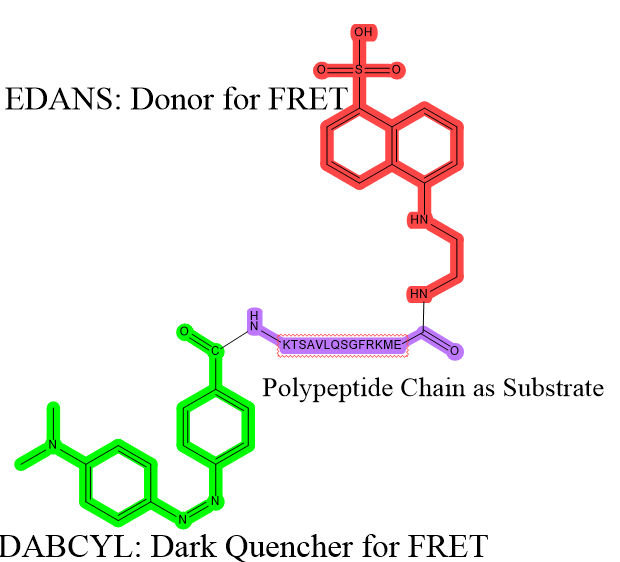
\includegraphics[width=0.5\linewidth]{../Figures/fluorescent substrate.png}
    \caption{Structure of Fluorescent Substrate}
    \label{Structure of Fluorescent Substrate}
\end{figure}

The overall consequence is that, when the substrate is consumed, then, it will show fluorescence.
Further process of reaction will lead to more intensive fluorescence which can be detected by \textbf{ELISA} in the unit of RFU.

\subsection{Detecting Half-maximal Inhibitory Concentration}
\begin{figure}
    \centering
    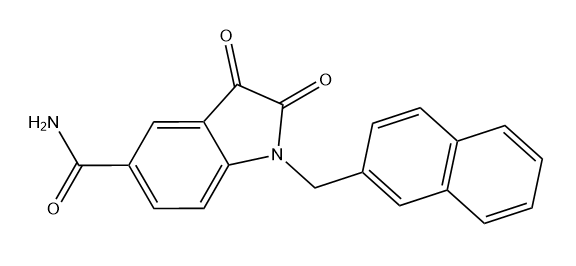
\includegraphics[width=0.5\linewidth]{../Figures/inhibitor structure.png}
    \caption{Structure of Inhibitor}
    \label{Structure of Inhibitor}
\end{figure}
The structure of inhibitor is shown in Figure \ref{Structure of Inhibitor}.
It will repress the reaction catalyzed by 3CL protease probably by competitive binding to the enzyme.
And we will determine the \textbf{Half-maximal Inhibitory Concentration, IC$_{50}$} through speed of reaction.

\section{Structure Detection: Structure Detection: CD Spectroscopy}
The secondary structure of protein can be assessed by \textbf{Circular Dichroism Spectroscopy (CD Spectroscopy)}\raisebox{5pt}{\tiny \cite{Lehninger}}.
The spectroscopy harnesses the differences in absorption of left-handed versus right-handed circularly polarized light.
As for the range of wave length, the far UV region (190 to 250 nm) is used to analysis.
The $\alpha$ helix and $\beta$ sheets have characteristic CD spectra due to their peptide bond folding states.

To completely define the secondary structure of polypeptide segment, we should also figure out the $\phi$ and $\psi$ angles of each amino acid residues.
The $\phi$ and $\psi$ stand for the important dihedral angles in a peptide.
\begin{align}
    \phi &= \text{dihedral}(C-N-C_{\alpha}-C)\\
    \psi &= \text{dihedral}(N-C_{\alpha}-C-N)
\end{align}

Two quantities are often used to describe the result: $\theta$, $\Delta \epsilon$ and $[\theta]$.
The transformation and definition of them are shown below:
\begin{align}
    \Delta \epsilon &= \epsilon_{L}-\epsilon_{R}\\
    \Delta A &= A_{L}-A_{R}\\
    \Delta A &= \Delta \epsilon \, l \, c\\
    [\theta] &= \frac{100\theta}{lcN_{\text{amino acid residues}}}\\
    \tan \theta &= \frac{E_{R} - E_{L}}{E_{R} + E_{L}} \approx \theta\\
    \theta &\approx \frac{\sqrt{I_{R}} - \sqrt{I_{L}}}{\sqrt{I_{R}} + \sqrt{I_{L}}}\\
    \theta &\approx \Delta \epsilon \, l \, c \times \frac{\ln 10}{4} \times \frac{180}{\pi}
\end{align}
In the above equations, $\theta$ is called ellipticity ,$[\theta]$ is \textbf{mean residue molar ellipticity} and $\Delta \epsilon$ is \textbf{molar circular dichroism}.
\section{Thermodynamic Parameters Measuring}
\textbf{Isothermal Titration Calorimetry (ITC)} is used to determine thermal dynamic parameters including enthalpy, entropy, equilibrium constant.
During the measurement, both reference cell and sample cell are heated to maintain the constant temperature while the input of heat impulse will be recorded precisely for calculation.

The procedure and logic behind it are as following:
\begin{itemize}
    \item Figure out the stoichiometric ratio N according to the corresponding position of maximal slope.
    \item Determine $\Delta$H from the difference between final and initial heat.
    \item Fit the curve to get the equilibrium constant K (corresponds to the value of maximal slope).
    \item Calculate $\Delta G=-RT\ln K$
    \item Calculate $\Delta S$ by the definition of $\Delta G=\Delta H -T\Delta S$.
\end{itemize}
\section{Model of Protein Binding}
\subsection{Virtual Screening: By Molecular Docking}
We use the method of \textbf{Molecular Docking} to predict the binding orientation and affinity of twenty different Ligands, which is able to achieve enough accuracy with a relatively short period.
The docking engine chosen by us is AutoDock Vina.
\subsection{Interaction Analysis}
After determining the most suitable ligand, I analyzed the interaction between the ligand and receptor in PyMOL with the purpose of providing an interpretation of its strong affinity. 

\chapter{Experimental Process}
\section{Protein Purification}
\subsection{\textit{E.coli} Lysis: Homogenizer}
\subsubsection{Materials}
\begin{itemize}
    \item Buffer Lysis
    \begin{itemize}
        \item PBS (Phosphate Buffered Saline: \ce{HPO_4^2- / H2PO_4-}): 20 mM (pH=7.3)
        \item \ce{NaCl}: 500 mM
        \item Imidazole: 10 mM
        \item DTT (Dithiothreitol: Reducing Agent): 1 mM
        \item PMSF (Phenylmethanesulfonyl Fluoride: Serine Protease Inhibitor): 1 mM
    \end{itemize}
\end{itemize}
\subsubsection{Procedure}
\begin{itemize}
    \item Stir the buffer lysis containing \textit{E.coli} until without obvious lumps and precipitates in an ice bath.
    \item Filter the mixture (50 mL) by gauze and then pour into the \textbf{homogenizer}\raisebox{5pt}{\tiny \cite{Homogenization}} with 10 mL \ce{H2O} following the below settings:
    \begin{itemize}
        \item Raise the pressure to 1,000 bar for 2 minutes.
        \item Pause 1 minute.
        \item Repeat the cycle 3 times.
    \end{itemize}
    \item Centrifugate the liquid at 14,000 rpm for 30 minutes.
    \item Strain the product through a filter (0.45 $\upmu$m) into a graduated cylinder.
\end{itemize}
\subsection{Affinity Chromatography: Immobilized \ce{Ni^2+} Metal Ion + His-tag}
\subsubsection{Materials}
\begin{itemize}
    \item Buffer A
    \begin{itemize}
        \item PBS (Phosphate Buffered Saline: \ce{HPO_4^2- / H2PO_4-}): 20 mM (pH=7.3)
        \item \ce{NaCl}: 500 mM
        \item Imidazole: \textbf{10 mM}
    \end{itemize}
    \item Buffer B
    \begin{itemize}
        \item PBS (Phosphate Buffered Saline: \ce{HPO_4^2- / H2PO_4-}): 20 mM (pH=7.3)
        \item \ce{NaCl}: 500 mM
        \item Imidazole: \textbf{500 mM}
    \end{itemize}
    \item Buffer C
    \begin{itemize}
        \item PBS (Phosphate Buffered Saline: \ce{HPO_4^2- / H2PO_4-}): 40 mM (pH=7.3)
        \item \ce{NaCl}: 100 mM
        \item EDTA: 1 mM
    \end{itemize}
\end{itemize}
\subsubsection{Procedure}
We purified 3CL protease fist by affinity chromatography.
Immobilized \ce{Ni^2+} ion had been attached to the column while His-tag (six histidine in the terminal of protein) had been fused with 3CL protease.

The \ce{Ni^2+} column has the capacity of 5 mL.
We washed the column before loading using buffer A and buffer B in turn (A(25 mL)-B(25 mL)-A(15 mL)-B(15 mL)-A(15 mL)) as shown in the blue curve in Figure \ref{Affinity Chromatography: UV Absorbance} and Figure \ref{Affinity Chromatography: Conductance}.
We set pressure difference ($\Delta P=0.3$ MPa) to be the control threshold with the pre-column pressure ($P_{pre}=0.5$ MPa).
The flow rate was set to be 1 mL/min for above operation.

Then we loaded 55 mL sample after lysis into the column with the flow velocity to be 2 mL/min.
After that, buffer A was constantly pumped into to column to elute impurities until the signal of UV absorbance went back near 0 mAU.
Once the eluting was complete, we started to raise the proportion of buffer B linearly to form a linear gradient.
The threshold of scope to collect product was set to be 20\% buffer elution (within the 0\% to 100\% buffer elution gradient).
The fraction collecting was performed automatically with the amount of 1.8 mL/tube.
Finally, we collected tubes from number 3 to number 8, totally $6\times1.8=10.8$ mL.

Condensation with centrifuging filtering and solvent changing was used condense 10.8 mL solution to nearly 1.5 mL.
The centrifuging was in 4$^\circ$C with the rotating speed of 3,500 rpm for 10 minutes.
In each turn, we decanted 5 mL solvent for the Gel-filtration Column to replace the buffer for \ce{Ni^2+} column containing lots of imidazole.
\subsection{Gel-filtration Chromatography}
\subsubsection{Procedure}
The Gel-filtration Column has the capacity of 24 mL.
We set pressure difference ($\Delta P=1.8$ MPa) to be the control threshold with the pre-column pressure ($P_{pre}=5.0$ MPa).
Careful washing of the column and sample ring was performed.
As for the sample ring, 4 mL ultra-pure water with 4 mL buffer assay were used to wash the pipe.
The two direction of washing(up to down and vice versa) with careful injector operation was included to ensure any bubble would be excluded from the column.

The loading amount should be 500 $\upmu$L with the concentration of 1 mg/mL.
To ensure the sample concentration to be around 1 mg/mL, we detected the concentration of the sample by nano drop.
The result was 6.737 Abs equivalent to $6.737\times1.07=7.21$ mg/mL.
That means around 70 $\upmu$L concentrated protease was needed with 430 $\upmu$L buffer assay.
However we enlarged the system by two fold which means diluting 140 $\upmu$L concentrated protease with 860 $\upmu$L buffer assay in case of failure.



We collected according to the UV absorbance as shown in Figure \ref{Gel-filtration Chromatography: UV absorbance with Conductace} and Figure \ref{Gel-filtration Chromatography: UV absorbance with Percentage of Buffer B}.
Then condensed the sample as previous process in affinity chromatography.

\begin{align}
    A &= \epsilon cl \\
    A &= 6.737\ Abs \\
    \epsilon &= 0.937\ \text{L/g}\cdot\text{cm} \\
    l &= 1\ \text{cm}\\
    c &\approx 7.21\ \text{mg/mL}=\frac{7.21\ \text{g/L}}{34\times 10^3 \text{g/mol}}=212.1\ \upmu\text{M}    
\end{align}


\subsection{Analyzing: SDS-PAGE}

\subsubsection{Procedure}
In this experiment, we used precast polyacrylamide gel.
However, we still need to prepare the buffer(500 mL) for electrophoresis by hands.

Four type of samples were prepared for SDS-PAGE to check the effect of protein purification.

\begin{itemize}
    \item No.1 \textit{E.coli} lysate
    \item No.2 Supernate of lysate after centrifuging
    \item No.3 Sample after affinity chromatography
    \item No.4 Sample after gel-filtration chromatography
\end{itemize}

In each well, we put 20 $\upmu$L sample with 5 $\upmu$L loading buffer except for No.3 which only left 8 $\upmu$L.
To control the concentration in consistency, only 2 $\upmu$L loading buffer was added to No.3.

We mixed the solution by \textbf{Vortex Genie 2} and centrifuge for instant.
Then heated at 94 $^\circ$C for 3 minutes.
Finally, loaded marker (2 $\upmu$L) as well as the four types of sample (10 $\upmu$L) into the polyacrylamide gel in sequence.

The electrophoresis apparatus was set at 150 V working for 38 minutes.

After electrophoresis, the gel was stained using Coomassie Brilliant Blue with heating in microwave oven for three times.
In each turn, the paint was heated until boiling.
3\% Acetic acid-\ce{H2O} was used to destain with the similar procedure in microwave oven.

\section{Enzyme Kinetics}
% Table
\begin{table}
    \centering
    \caption{Substrate Solution Configuration in Microplate}
    
    \begin{tabular}{|c|c|c|c|c|c|c|c|c|} \hline
        Number of Sample&1&2&3&4&5&6&7&8 \\ \hline
        Substrate Concentration ($\upmu$M)&500&750&1000&1250&1500&2000&2500&3000 \\ \hline
        DMSO Solvent ($\upmu$L)& 9&8.5&8&7.5&7&6&5&4\\ \hline
        5000$\upmu$M Concentrated Substrate ($\upmu$L)&1&1.5&2&2.5&3&4&5&6 \\ \hline
    \end{tabular}
    \label{Substrate Solution Configuration in Microplate}
\end{table}
\begin{figure}
    \centering
    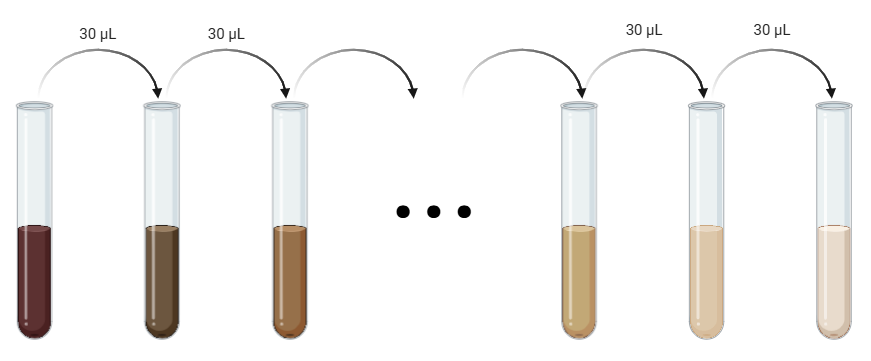
\includegraphics[width=0.7\linewidth]{../Figures/serial dilution.png}
    \caption{Serial Dilution of Inhibitor}
    \label{Serial Dilution of Inhibitor}
\end{figure}
\begin{figure}
    \centering
    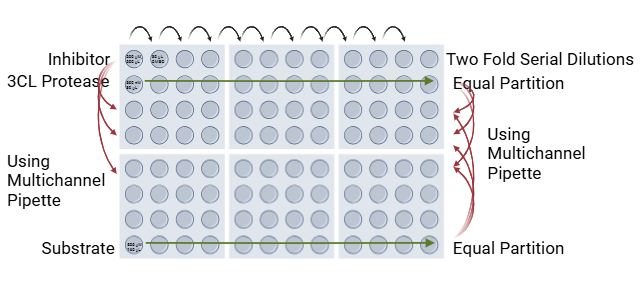
\includegraphics[width=1\linewidth]{../Figures/microplate.png}
    \caption{Solution Configuration in Microplate}
    \label{Inhibitor Solution Configuration in Microplate}
\end{figure}
The following experiments involve tedious configuration of solutions with different concentrations, including substrate, 3CL Protease (Enzyme), and inhibitor.
To summarize and visualize the complicated process of dilution, I have drawn the Figure \ref{Inhibitor Solution Configuration in Microplate}.
Generally speaking, we used \textbf{multichannel pipette} to transfer a whole row of solution to other three different rows because of the three independent parallel groups.
Before that, however, we must use \textbf{single-channel pipette} to adjust the concentration in one row.
The \textbf{two fold serial diluting}, as shown in Figure \ref{Serial Dilution of Inhibitor}, was used for inhibitor while substrate was diluted one by one differently as shown in Table \ref{Substrate Solution Configuration in Microplate}.

\subsection{Verifying Michaelis Menton Equation}
\subsubsection{Procedure}

The independent variable in Michaelis Menton Equation is the concentration of substrate $[S]$.
Thus to verify the equation we must configure the substrate solution of different concentrations.
We started by dissolving 2 mg solid substrate into 192 $\upmu$L DMSO solvent, which has the concentration of 5000 $\upmu$M.
Then, we adjusted the ratio of DMSO and concentrated substrate to achieve 8 different concentrations of substrate solution, as shown in Table \ref{Substrate Solution Configuration in Microplate}.

The Composition of the System (100 $\upmu$L):
\begin{itemize}
    \item Buffer Assay (80 $\upmu$L, 80\%)
    \begin{itemize}
        \item \ce{Na2HPO4 / NaH2PO4} (40 mM)
        \item \ce{NaCl} (100mM)
        \item \ce{EDTA} (1mM)
        \item Triton X-100 (0.1\%)
    \end{itemize}
    \item SARS-CoV2-3CL Protease (10 $\upmu$L, 10\%) (before mixing: 500 nM, after mixing: 50 nM)
    \item Fluorescent Substrate (10 $\upmu$L, 10\%) (before mixing the different concentrations can be seen in Table \ref{Substrate Solution Configuration in Microplate}).
    \item Temperature: 25$^\circ$C
\end{itemize}

3CL protease was preserved in fridge at -80$^\circ$C, which was then melted in ice box.
The initial concentration of 3CL protease was 206 $\upmu$M, and then we took 2 $\upmu$L diluting it with 2 mL Buffer Assay to get 500 nM protease solution.
The buffer assay was prepared by adding 50 $\upmu$L Triton X-100 into 50 mL buffer solution at the very beginning.

Both buffer assay and 3CL protease were partitioned equally into eight different wells in the same microplate, and were mixed using multichannel pipette in other three rows.
Fluorescent substrate was stored in another microplate while was prepared according to Table \ref{Substrate Solution Configuration in Microplate}.
Also, multichannel pipette was used to transfer substrate into the system.

We detected the speed of reaction by the concentration variation of fluorescent substrate which was identified by \textbf{enzyme-linked immunosorbent assay (ELISA)}.
The original data is shown in Figure \ref{Reaction Rate versus Substrate Concentration: 8 groups of experiments}.

\subsection{Detecting Half-maximal Inhibitory Concentration}
\subsubsection{Procedure}
The inhibitor is consist of competitive inhibitor, uncompetitive inhibitor and mixed inhibitor.
Instead of changing substrate concentration simultaneously, we varied inhibitor concentration [I] only and keep [S] under control.
Also, we focused on \textbf{Half-maximal Inhibitory Concentration (IC$_{50}$)} only, without concerns about modified factors to $V_{max}$ or $K_m$.

The following procedure was used to prepare to inhibitor solution with different concentration:

% List
\begin{itemize}
    \item sample 20 $\upmu$L concentrated inhibitor(20 mM) solution with 180 $\upmu$L DMSO as additional solvent. Then mix in $1^{st}$ well of microplate, which has the concentration of 200 $\upmu$M.
    \item prepare 30 $\upmu$L DMSO in each well of $1^{st}$ raw.
    \item take 30 $\upmu$L solution from $1^{st}$ to $2^{nd}$ and mix in $2^{nd}$ well.
    \item repeat the step for the following wells to perform two fold serial dilution as shown in Figure \ref{Serial Dilution of Inhibitor}.
\end{itemize}

To get the solution of substrate, we decanted 1.92 mL DMSO into 2 mg fluorescent substrate then separated it into twelve different wells in the same row.
As shown in Figure \ref{Inhibitor Solution Configuration in Microplate}, the substrate and inhibitor were in different rows.
To be noted that, in reality, they were also stored in separated microplates to avoid unwanted illumination of fluorescent substrate.

The Composition of the System (100 $\upmu$L):
\begin{itemize}
    \item Buffer Assay (80 $\upmu$L, 80\%)
    \begin{itemize}
        \item \ce{Na2HPO4 / NaH2PO4} (40 mM)
        \item \ce{NaCl} (100mM)
        \item \ce{EDTA} (1mM)
        \item Triton X-100 (0.1\%)
    \end{itemize}
    \item SARS-CoV2-3CL Protease (10 $\upmu$L, 10\%) (before mixing: 500 nM, after mixing: 50 nM)
    \item Fluorescent Substrate (5 $\upmu$L, 5\%) (before mixing: 500 $\upmu$M, after mixing: 25 $\upmu$M)
    \item Inhibitor (5 $\upmu$L, 5\%) (after mixing the serial concentration can be seen in Figure \ref{Reaction Rate versus Inhibitor Concentration: 12 groups of experiments, each has 3 parallel groups}).
    \item Temperature: 25$^\circ$C
\end{itemize}

\section{Structure Detection: Structure Detection: CD Spectroscopy}
\subsubsection{Materials}
\begin{itemize}
    \item CD Buffer (pH=7.4): \ce{KH2PO4} 20 mM 19.8 mL + \ce{K2HPO4} 20 mM 80.2 mL
    \item Guanidinium Chloride 12M
    \item Protein Solution 2 mg/mL 
\end{itemize}
\subsubsection{Procedure}
We took the measurement from the wavelength of 190 nm to 340 nm in the cuvette with light path equals 10 mm.
The corresponding sample (protein+guanidine) dosage is 2 mL where 1 mL coming from 2 mg/mL protein the other 1 mL coming from diluted guanidinium chloride.
Therefore, we diluted and mixed the protein with guanidine according to the Table \ref{Configuration of Solution for CD Spectroscopy}.
\begin{table}
    \centering
    \caption{Configuration of Solution for CD Spectroscopy}
    \label{Configuration of Solution for CD Spectroscopy}
    \begin{tabular}{|c|c|c|c|c|}
        \toprule
        No. & Guanidine Final Concentration (M) & Guanidine Volume (mL) & CD Buffer (mL) & Protein (mL) \\
        \midrule
        1 & 1.2 & 0.2 & 0.8 & 1 \\
        2 & 2.4 & 0.4 & 0.6 & 1 \\
        3 & 3.6 & 0.6 & 0.4 & 1 \\
        4 & 4.8 & 0.8 & 0.2 & 1 \\
        5 & 6.0 & 1.0 & 0.0 & 1 \\
        \bottomrule
    \end{tabular}
\end{table}

Before measuring we installed the apparatus and filling the light path with \ce{N2}.
The mixture of guanidinium chloride with protein was put in ice box for 1 minute to denature the protein.
However we adapted the more practical control of time by limiting the whole process, including adding protein to cuvette then guanidine, to be 3 minutes.
Finally we took measurement for five different samples.

\section{Thermodynamic Parameters Measuring}
For practical purposes, we chose the reaction of \ce{MgCl2} and \ce{EDTA} to be measured instead of the binding of inhibitor with protein.
The measurements were performed twice under 25$^\circ$C and 30$^\circ$C respectively with the parameters shown in Table \ref{Experimental Parameters of ITC}.

Since most of the steps were performed automatically, the only process that remained difficult was loading or injecting the solution into the cells.
Strict 280 $\upmu$L was injected into the cells confirmed by the steady curve in the initial delay period.
\begin{table}
    \centering
    \caption{Experimental Parameters of ITC}
    \label{Experimental Parameters of ITC}
    \begin{tabular}{|c|c|}
        \toprule
        Total Injections & 16 \\
        \midrule
        Cell Temperature ($^\circ$C) & 25 and 30 \\
        Preference Power (pCal/sec) & 11 \\
        Initial Delay (sec) & 60 \\
        Syringe Concentration (mM) & 5 \\
        Cell Concentration (mM) & 0.40 \\
        Stiring Speed (rpm) & 1000 \\
        \bottomrule
    \end{tabular}
        
        
\end{table}
\section{Model of Protein Binding}
\subsection{Virtual Screening: By Molecular Docking}
We used AutoDock Vina to be the docking engine for the experiment, which had been installed on our laptops' linux environment (windows subsystem).
There were twenty ligand candidates to be the inhibitor and we would choose the one having maximal binding affinity.
To perform molecular docking in Vina, a key step was determining the center and size of vina box for searching.
I uploaded the 7EN8 protein data to the website called CAVITYPLUS\raisebox{5pt}{\tiny \cite{pkumdl}} to get box size and box center which corresponds to the binding pocket of the protein.

I screened the inhibitor according to the maximal binding affinity of each ligand.

\subsection{Interaction Analysis}
After selecting the most suitable ligand out, I observed the ligand and receptor in the software called PyMOL.
The nearby residues surrounding the ligand were kept while irrelevant residues were hidden for clarify.
Given the type of amino acid residues and the distance and conformation, I can deduce the interaction between the ligand and receptor.

\chapter{Results and Discussion}
\section{Protein Purification}
\subsection{\textit{E.coli} Lysis: Homogenizer}
As the initial step, homogenization must succeed, which was proved by the subsequent results.
However, for the homogenization itself, the clarifying solution was the indication of success.
\subsection{Column Chromatography}
\subsubsection{Affinity Chromatography: Immobilized \ce{Ni^2+} Metal Ion + His-tag}
The tracking of UV absorbance changing and conductance changing with varied buffer B proportion can be seen in Figure \ref{Affinity Chromatography: UV Absorbance} and Figure \ref{Affinity Chromatography: Conductance}.
The major peak in the middle of the Figure \ref{Affinity Chromatography: UV Absorbance} corresponds to the impurities (protein that has UV absorbance companied by nucleic acid).
Meanwhile the conductance drops down (Figure \ref{Affinity Chromatography: Conductance}) due the poor conductivity of protein compared with inorganic salts.

From the Fourth Column in Figure \ref{Results of SDS-PAGE} we can clearly see the effective purification produced by affinity chromatography compared with the lysis mixture in second and third column.

\begin{figure}
    \centering
    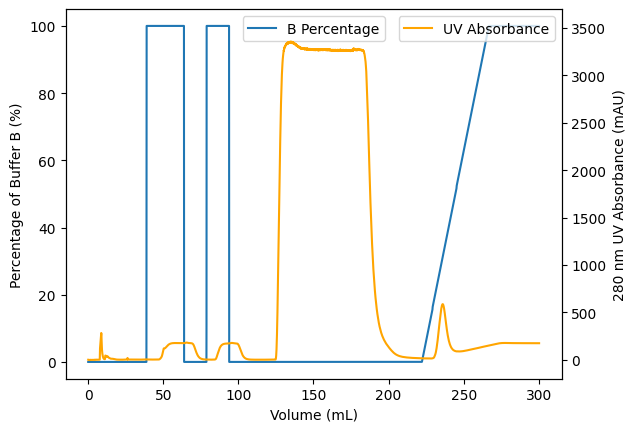
\includegraphics[width=0.6\linewidth]{../Figures/Affinity Column UV.png}
    \caption{Affinity Chromatography: UV Absorbance with Percentage of Buffer B}
    \label{Affinity Chromatography: UV Absorbance}
\end{figure}

\begin{figure}
    \centering
    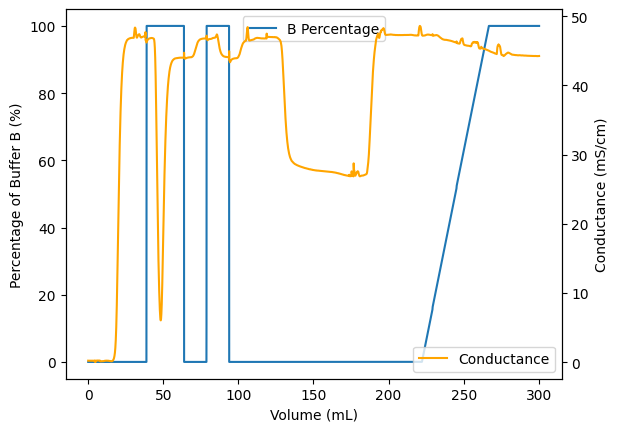
\includegraphics[width=0.6\linewidth]{../Figures/Affinity Column Conductance.png}
    \caption{Affinity Chromatography: Conductance with Percentage of Buffer B}
    \label{Affinity Chromatography: Conductance}
\end{figure}
\subsubsection{Gel-filtration Chromatography}
The effect can be seen in Figure \ref{Results of SDS-PAGE}.
Compared with the fourth column, the last column after gel-filtration chromatography does not show additional purification.
Probably, the solution had been purified to an extreme extend after affinity chromatography, which leads to the unobvious improvement.

Besides, the molecular weight can be estimated according to the volume where we observed the peak of UV absorbance in Figure \ref{Gel-filtration Chromatography: UV absorbance with Conductace}.
The UV peak locates near 10.1 mL, and therefore the molecular weight is around 43 kDa (between 13.7 kDa to 43 kDa), which is consistent with the more exact result gotten from SDS-PAGE as following.
$$
\text{molecular weight}\approx 43 \ \text{kDa (according to Gel-filtration Chromatography)}
$$
\begin{figure}
    \centering
    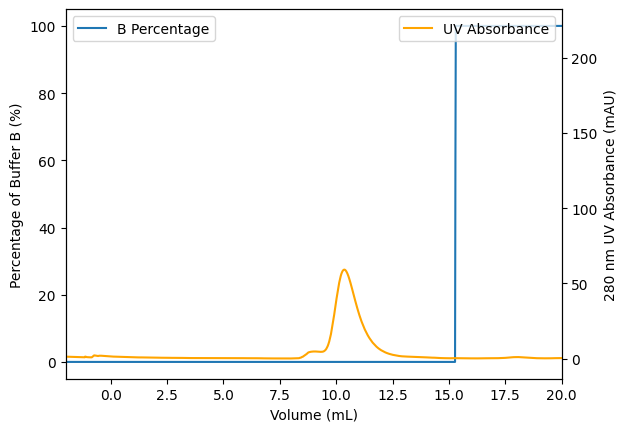
\includegraphics[width=0.6\linewidth]{../Figures/Filtration Column UV.png}
    \caption{Gel-filtration Chromatography: UV absorbance with Percentage of Buffer B}
    \label{Gel-filtration Chromatography: UV absorbance with Percentage of Buffer B}
\end{figure}

\begin{figure}
    \centering
    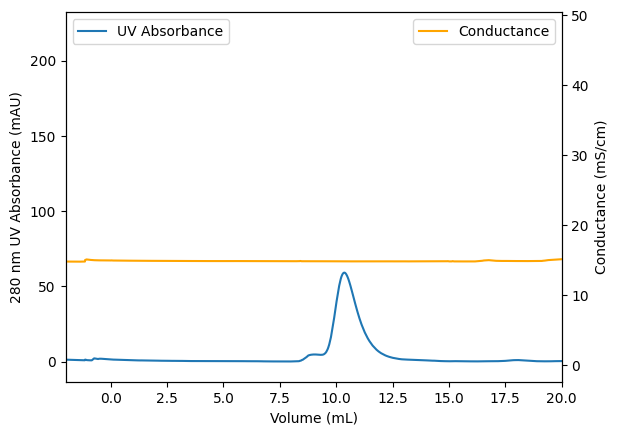
\includegraphics[width=0.6\linewidth]{../Figures/Filtration Column UV and Conductance.png}
    \caption{Gel-filtration Chromatography: UV absorbance with Conductance}
    \label{Gel-filtration Chromatography: UV absorbance with Conductace}
\end{figure}


\subsection{Analyzing: SDS-PAGE}
\begin{figure}
    \centering
    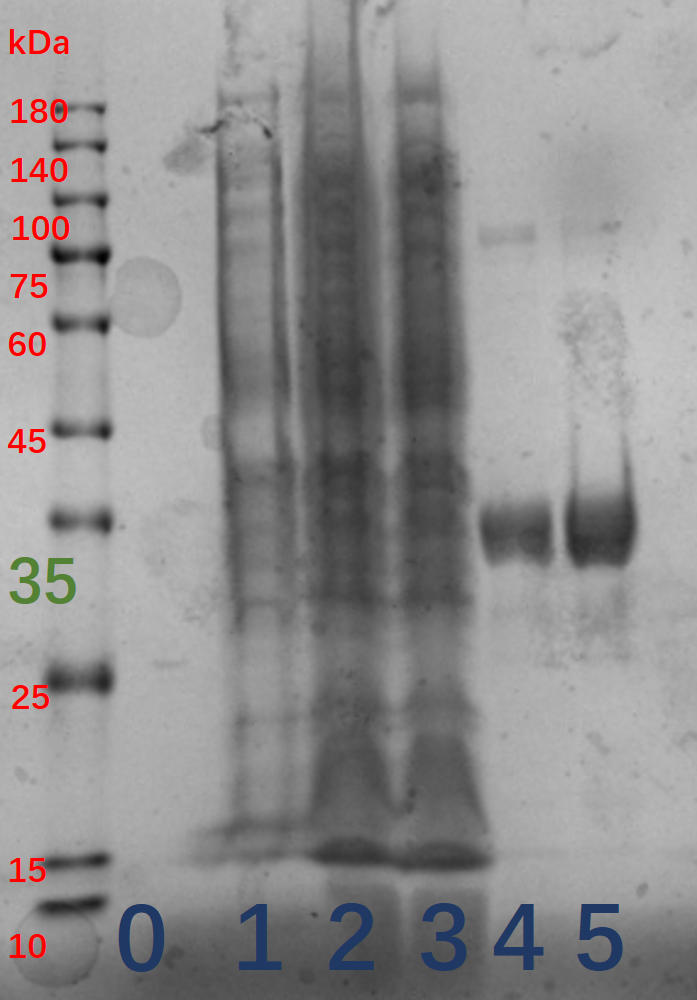
\includegraphics[width=0.7\linewidth]{../Figures/SDS-PAGE.png}
    \caption{Results of SDS-PAGE: The Second Column is the solution after lysis; The Third Column is from supernate; The Fourth Column is after affinity chromatography; The Last One is after gel-filtration chromatography. The First Column has the same composition as the second one just with additional loading buffer. The leftmost one is marker.}
    \label{Results of SDS-PAGE}
\end{figure}
As shown in Figure \ref{Results of SDS-PAGE}, the effect of purification is obvious.
The most effective method should be affinity chromatography while other steps are also playing an important role in the whole process.
Besides, we can also figure out the molecular weight of 3CL protease which is near \textbf{34 kDa}.
$$
\text{molecular weight}\approx 34 \ \text{kDa (according to SDS-PAGE)}
$$
The result of 34 kDa should be more accurate than the one obtained from Gel-Filtration Chromatography above.
\section{Enzyme Kinetics}
\subsection{Verifying Michaelis Menton Equation}
The original data gotten from \textbf{ELISA} is visualized in Figure \ref{Reaction Rate versus Substrate Concentration: 8 groups of experiments}.
In each subfigure, I have drawn the three parallelled groups of same substrate concentration.
It should be noted that, the several initial points were omitted for keeping linear parts only in accordance with the assumptions of Michaelis Menton Equation (the [ES] has reached steady state, not changing with time).

I performed linear regression to each of them, then averaged the slope which represents the speed of reaction.

The eight slopes (speed of reaction) were plotted with respect to substrate concentration [S] then.
As shown in Figure \ref{Reaction Rate versus Substrate Concentration: in normal axes}, the consequence is a curve which was similar to the prediction of Michaelis Menton Equation.

To further analyze the results, however, I converted the axes to the reciprocal of speed $V_0^{-1}$ and substrate concentration $[S]^{-1}$.
The benefit of reciprocal plotting is that we can operate linear regression again.
$$
\frac{1}{V_0}=\frac{K_m}{V_{max}}\cdot \frac{1}{[S]}+\frac{1}{V_{max}}\\
$$
$$
y=kx+b
$$
The vertical intercept b is $\frac{1}{V_{max}}$ and the horizontal intercept corresponds to $-\frac{1}{K_m}$, which are also annotated in Figure \ref{Reaction Rate versus Substrate Concentration: in reciprocall axes}.

$$
V_{max}=20 \ \text{RFU/second}
$$

$$
K_{m}=28.99 \ \upmu \text{M}
$$


\begin{figure}
    \centering
    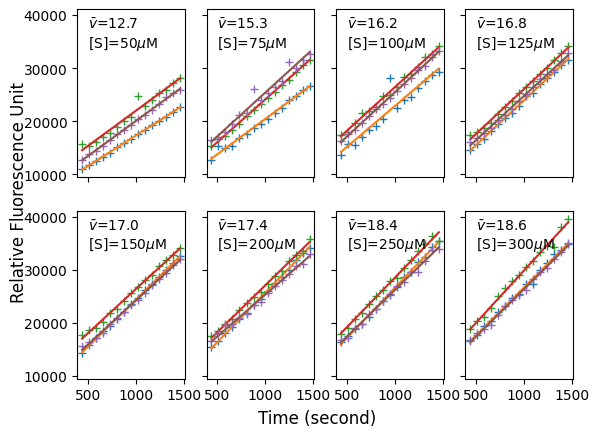
\includegraphics[width=0.5\linewidth]{../Figures/substrate1.png}
    \caption{Reaction Rate versus Substrate Concentration: 8 groups of experiments, each has 3 parallel groups}
    \label{Reaction Rate versus Substrate Concentration: 8 groups of experiments}
\end{figure}

\begin{figure}
    \centering
    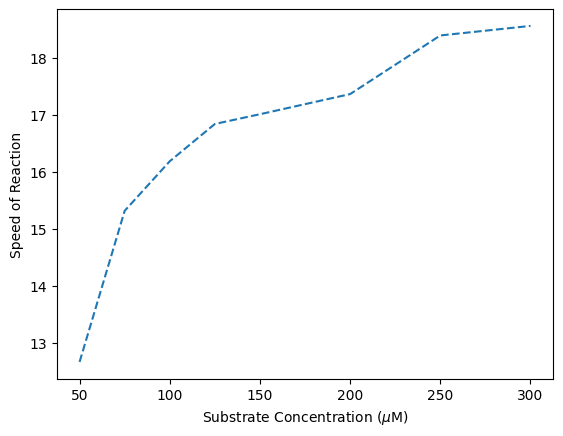
\includegraphics[width=0.5\linewidth]{../Figures/substrate2.png}
    \caption{Reaction Rate versus Substrate Concentration: in normal axes}
    \label{Reaction Rate versus Substrate Concentration: in normal axes}
\end{figure}

\begin{figure}
    \centering
    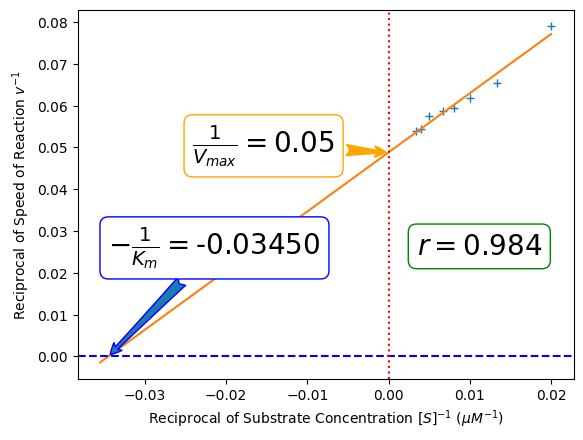
\includegraphics[width=1\linewidth]{../Figures/substrate3.png}
    \caption{Reaction Rate versus Substrate Concentration: in reciprocal axes}
    \label{Reaction Rate versus Substrate Concentration: in reciprocall axes}
\end{figure}

\subsection{Detecting Half-maximal Inhibitory Concentration}
The reaction speed was also detected by \textbf{ELISA}.
Twelve subfigures are shown in Figure \ref{Reaction Rate versus Inhibitor Concentration: 12 groups of experiments, each has 3 parallel groups} and each of them corresponds to a different inhibitor concentration [I].
There are two intriguing phenomena in the figure.
Firstly, one group in [I]=10 $\upmu$M and one group in [I]=1.25 $\upmu$L exist extreme fluctuations which may caused by bubbles in solution.
Secondly, the reaction speed has negative value in high concentration of inhibitor.
The major cause of that absurd phenomenon is probably the unsteady state with fluctuation at early initial period.
To eliminate the negative value and disturbance of it, I also decided to omit the early four points, which should reasonable and appropriate.


\begin{figure}
    \centering
    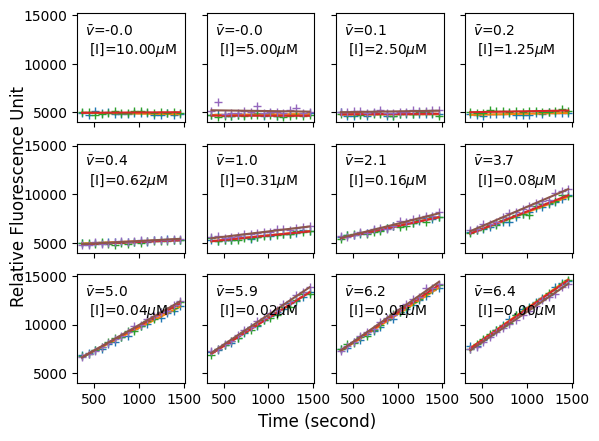
\includegraphics[width=1\linewidth]{../Figures/inhibitor1.png}
    \caption{Reaction Rate versus Inhibitor Concentration: 12 groups of experiments, each has 3
    parallel groups}
    \label{Reaction Rate versus Inhibitor Concentration: 12 groups of experiments, each has 3
    parallel groups}
\end{figure}

I performed linear regression again to each group and average the parallel groups to get the mean speed of reaction.
Then the plot of mean speed $\bar{V_0}$ versus inhibitor concentration was drawn.
From Figure \ref{Reaction Rate versus Inhibitor Concentration: determining IC50}, we can identify the \textbf{Half-maximal Inhibitory Concentration IC$_{50}$}, which is IC$_{50}=0.095\ \upmu \text{M}$.
Somehow, the value is higher than the reported value IC$_{50}=0.095\ \upmu \text{M}$.

$$
\text{IC}_{50}=0.095\ \upmu \text{M}
$$

The IC$_{50}=0.095\ \upmu \text{M}$ measured by us was twice as the reported value IC$_{50}=0.045\ \upmu \text{M}$, which may be caused by slightly different experimental conditions or by partial inefficiency of inhibitor solution.
\begin{figure}
    \centering
    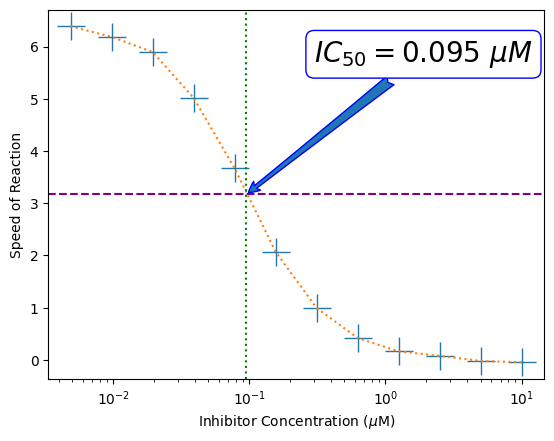
\includegraphics[width=1\linewidth]{../Figures/inhibitor2.png}
    \caption{Reaction Rate versus Inhibitor Concentration: determining $\text{IC}_{50}$}
    \label{Reaction Rate versus Inhibitor Concentration: determining IC50}
\end{figure}

Besides, we can also figure out the inhibitory rate with different inhibitory concentration [I].
The intuitive recognition can be acquired in Figure \ref{Reaction Rate versus Inhibitor Concentration: determining IC50} while the precise values are shown in Table \ref{Inhibitory Rate with Different Inhibitor Concentration}.

\begin{table}
    \centering
    \caption{Inhibitory Rate with Different Inhibitor Concentration}

    \begin{tabular}{|c|c|c|}
        \toprule
         & Inhibitor Concentration ($\upmu$M) & Inhibitory Rate \\
        \midrule
        0 & 10.00 & 100.00 \% \\
        1 & 5.00 & 99.59 \% \\
        2 & 2.50 & 98.07 \% \\
        3 & 1.25 & 96.72 \% \\
        4 & 0.62 & 92.77 \% \\
        5 & 0.31 & 83.84 \% \\
        6 & 0.16 & 67.12 \% \\
        7 & 0.08 & 42.29 \% \\
        8 & 0.04 & 21.31 \% \\
        9 & 0.02 & 7.65 \% \\
        10 & 0.01 & 3.15 \% \\
        11 & 0.00 & 0.00 \% \\
        \bottomrule
        \end{tabular}
    \label{Inhibitory Rate with Different Inhibitor Concentration}            
        
\end{table}


\section{Structure Detection: Structure Detection: CD Spectroscopy}
The raw data gotten from CD spectrometer is shown in Figure \ref{CD Absorbance}.
Besides, we have already known the following parameters:

\begin{align}
\text{Number of Residues}&=306\text{ residues}+5\text{ histidines}=311\\
\text{Concentration}&=29.4\text{ }\upmu\text{M}\\
\text{Pathlength}&=1\text{ cm}
\end{align}


After submitting the raw data to the website\raisebox{5pt}{\tiny \cite{bestsel}} to get the proportion of different secondary structures (alpha helix and beta sheets) as shown in Figure \ref{Secondary Structure of 3CL Protease}, we still could not tell the differences between the five groups.
However, we could still figure out the influence of guanidinium chloride.


As shown in Figure \ref{CD Absorbance}, in the far-UV regin(190 nm to 260 nm), especially the peak near 240 nm, the CD absorbance (ellipticity) increased with guanidinium chloride concentration.
While, in the near-UV regin (250 nm-320 nm), especially the CD absorbance peak extending from 260 nm to 280 nm, decreased and eventually diminished with the increasing guanidinium chloride concentration.
This phenomena reflects the influence of guanidine to the secondary structure of protein, however, lacking of more concrete implication about the percentage of alpha-helix and beta-sheet.



To analyze the reasons of the phenomenon, we can observe the pie chart shown in Figure \ref{Secondary Structure of 3CL Protease}.
The proportion of alpha helix is rather small while the unstructured portion accounts for nearly half of the protein.
Thus, I deduced the denaturing of protein even in the absence of guanidine.
Besides, the CD spectroscopy could not provide extremely accurate measurement which could only verify assumptions rather than figure out the protein structure from bottom.



\begin{figure}
    \centering
    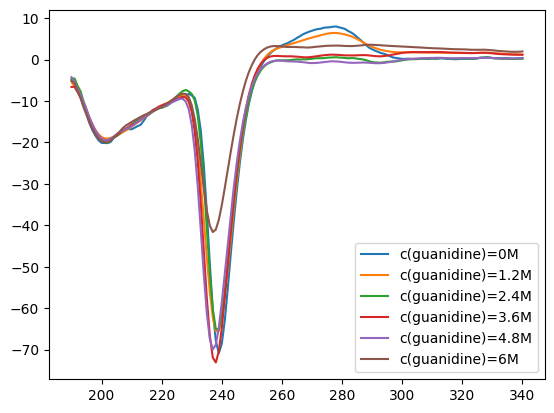
\includegraphics[width=0.8\linewidth]{../Figures/CD absorbance.png}
    \caption{CD Absorbance}
    \label{CD Absorbance}
\end{figure}
 % Figure
 \begin{figure}
    \centering
    \subfigure[guanidine=0 M]{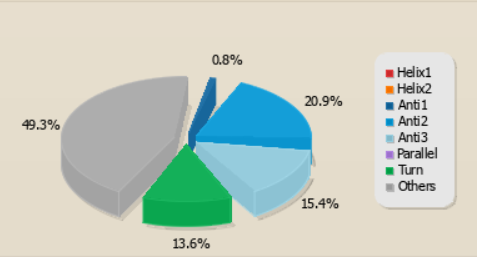
\includegraphics[width=0.3\linewidth]{../Figures/g0.png}}
    \subfigure[guanidine=1.2 M]{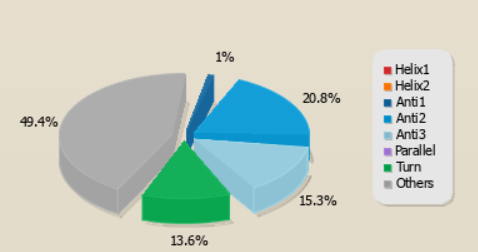
\includegraphics[width=0.3\linewidth]{../Figures/g12.png}}
    \subfigure[guanidine=2.4 M]{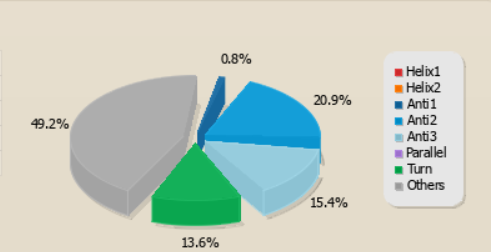
\includegraphics[width=0.3\linewidth]{../Figures/g24.png}}
    \subfigure[guanidine=3.6 M]{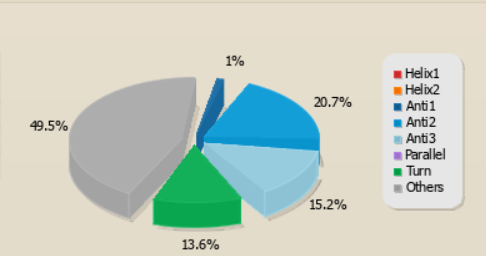
\includegraphics[width=0.3\linewidth]{../Figures/g36.png}}
    \subfigure[guanidine=4.8 M]{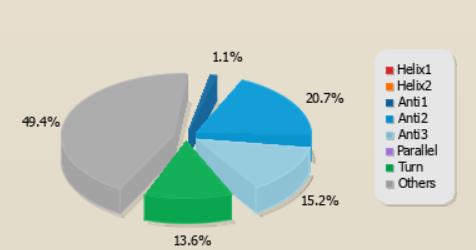
\includegraphics[width=0.3\linewidth]{../Figures/g48.png}}
    \subfigure[guanidine=6 M]{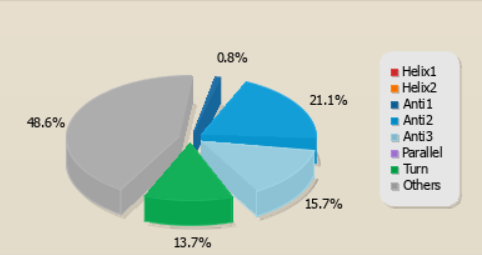
\includegraphics[width=0.3\linewidth]{../Figures/g60.png}}
    \caption{Secondary Structure of 3CL Protease with Different Guanidine Concentration}  
    \label{Secondary Structure of 3CL Protease}
 \end{figure}
\section{Thermodynamic Parameters Measuring}
The ITC  titration curve can be seen in Figure \ref{Titration Curve Measured by ITC}.
In the process of analysis, we neglect the second points because the large deviation must be caused by error rather than internal mechanism.
Based on the titration curve, the curve fitting was performed automatically, providing us with specific thermodynamic parameters as shown in Table \ref{Thermodynamic Parameters Measured by ITC}.
As for the reaction under consideration, $\Delta H$ has positive value indicating that the reaction absorbs heat from environment.
While the increasing equilibrium constant K with Temperature further confirmed the theory.

Besides, there is a small difference in the accuracy between the two group.
The group with high temperature ($30^\circ$C) has less error and higher accuracy, which is also intuitive.
In Figure \ref{Titration Curve Measured by ITC}, the $25^\circ$C group as negative slope at initial period which is not conform to thermal physical theory and must lead to less accuracy of measurement.
\begin{figure}
    \centering
    \subfigure[T=25$^\circ$C]{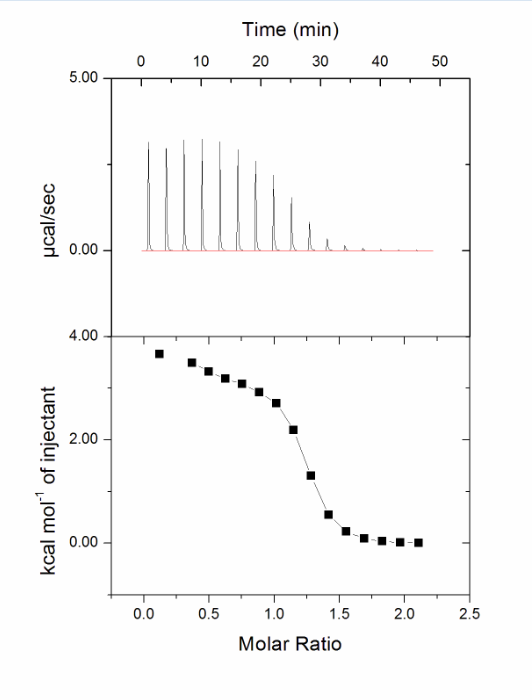
\includegraphics[width=0.45\linewidth]{../Figures/ITC25.png}}
    \subfigure[T=30$^\circ$C]{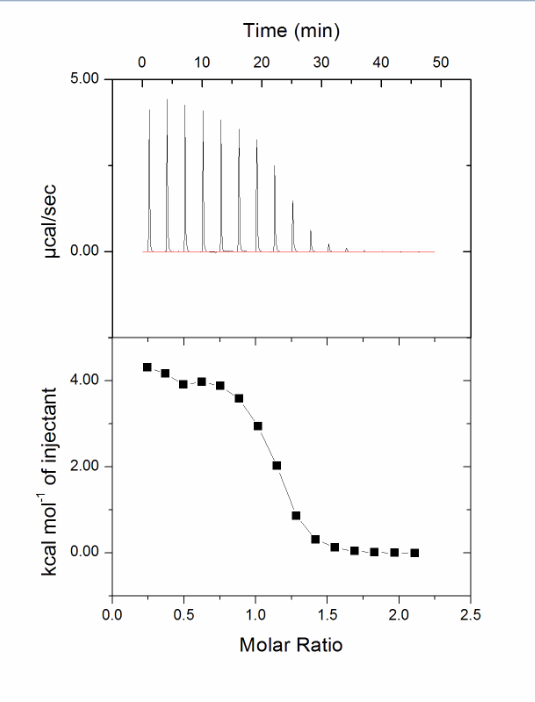
\includegraphics[width=0.45\linewidth]{../Figures/ITC30.png}}
    \caption{Titration Curve Measured by ITC}
    \label{Titration Curve Measured by ITC}
 \end{figure}
 \begin{table}
    \centering
    \caption{Thermodynamic Parameters Measured by ITC}
    \begin{tabular}{|c|c|c|}
        \toprule
        Temperature & 25$^\circ$C & 30$^\circ$C \\
        \midrule
        N & 1.16$\pm$0.0134 Sites & 1.07$\pm$0.00904 Sites \\
        K & $2.14\times 10^5\pm4.81\times10^4$ \text{M}$^{-1}$ & $2.70\times 10^5\pm4.49\times10^4$ \text{M}$^{-1}$ \\
        ΔH &3431$\pm67.69$ $\text{cal}\cdot\text{mol}^{-1}$ & 4160$\pm57.64$ $\text{cal}\cdot\text{mol}^{-1}$ \\
        ΔS &  35.9 $\text{cal}\cdot\text{mol}^{-1}\cdot\text{K}^{-1}$  & 38.6 $\text{cal}\cdot\text{mol}^{-1}\cdot\text{K}^{-1}$  \\
        \bottomrule
    \end{tabular}
    \label{Thermodynamic Parameters Measured by ITC}
 \end{table}

\begin{figure}
    \centering
    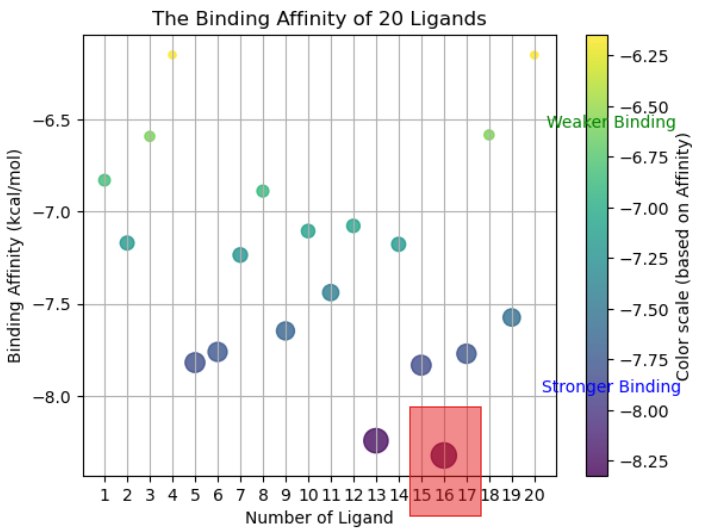
\includegraphics[width=0.8\linewidth]{../Figures/Virtual Screen.png}
    \caption{Virtual Screening of Ligand}
    \label{Virtual Screening of Ligand}
\end{figure}

\section{Model of Protein Binding}
\subsection{Virtual Screening: By Molecular Docking}
\begin{table}
    \caption{Binding Affinity of Ligands}
    \label{Binding Affinity of 20 Ligands}
    \centering
    \begin{tabular}{|c|c|}
        \toprule
        Number of Ligand & Affinity (kcal/mol) \\
        \midrule
        1 & -6.829 \\
        2 & -7.170 \\
        3 & -6.591 \\
        4 & -6.149 \\
        5 & -7.819 \\
        6 & -7.761 \\
        7 & -7.235 \\
        8 & -6.888 \\
        9 & -7.647 \\
        10 & -7.105 \\
        11 & -7.439 \\
        12 & -7.077 \\
        13 & -8.243 \\
        14 & -7.177 \\
        15 & -7.833 \\
        16 & -8.323 \\
        17 & -7.771 \\
        18 & -6.583 \\
        19 & -7.574 \\
        20 & -6.150 \\
        \bottomrule
        \end{tabular}        
      
\end{table}

According to the computing at pkumdl website\raisebox{5pt}{\tiny\cite{pkumdl}}, the center of vina box should be (-5.5, -7.75,26.25) with the size of (12.0, 15.5, 18.5).
$$
\text{center} = (-5.5, -7.75,26.25)
$$
$$
\text{size}= (12.0, 15.5, 18.5)
$$
The Table \ref{Binding Affinity of 20 Ligands} contains the binding affinity of each ligand while Figure \ref{Virtual Screening of Ligand} provides a visualization for it.
From both of them, we can easily pick out the most suitable ligands that is number 16 ligand.
\subsection{Interaction Analysis}
The overview of the ligand with receptor can be seen in Figure \ref{Interaction Analysis}.
Zooming in, we can observe in detail.
There are two major types of interaction between the ligand and receptor. One is hydrogen bond while the other one is pi-pi interaction.

As for the hydrogen bond, the amide group in the residue of glutamine in the 110 position provide hydrogen atom.
The H atom in the guanidino group of arginine at position of 298 is also the hydrogen donor for hydrogen bond.
The acceptor of hydrogen atoms are the oxygen atoms in ligand.

As for the pi-pi interaction, the approximation of phenylalanine at 294 position to the aromatic rings of the ligand indicates the existence of pi-pi interaction.
\begin{figure}
    \centering
    \subfigure[Ligand in the Pocket of Receptor]{
        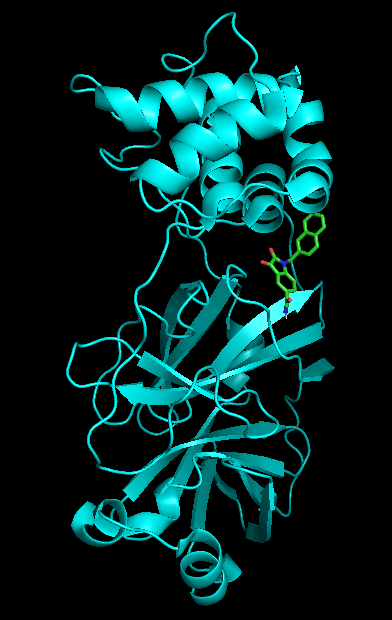
\includegraphics[width=0.4\linewidth]{../Figures/Receptor and Ligand 16.png}
    }
    \subfigure[Hydrogen Bond (Gln-110)]{
        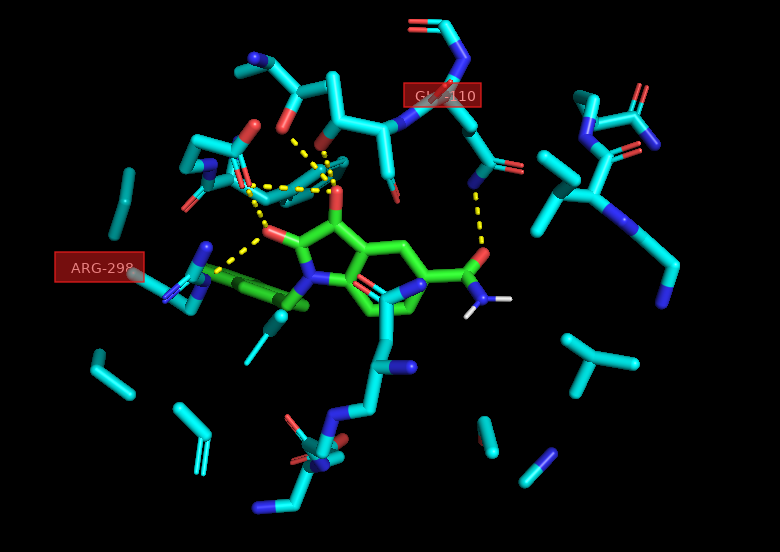
\includegraphics[width=0.4\linewidth]{../Figures/H-Bond.png}
    }
    \subfigure[Hydrogen Bond (Arg-298)]{
        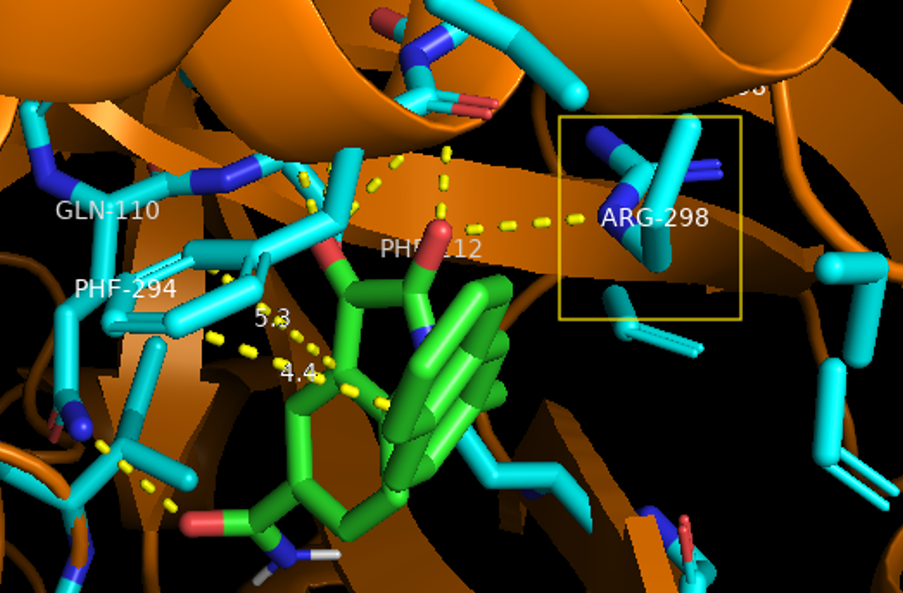
\includegraphics[width=0.4\linewidth]{../Figures/H-Bond-2.png}
    }
    \subfigure[pi-pi Interaction (Phe-294)]{
        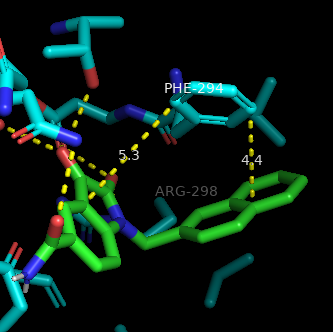
\includegraphics[width=0.4\linewidth]{../Figures/pi-pi interaction.png}
    }
    \caption{Interaction Analysis}
    \label{Interaction Analysis}
    
\end{figure}

\chapter{Conclusion}
I was amazed by the carefully designed experimental classes which walked us through the wonderful process of analyzing protein.
From my point of view, the set of experiments follows the logic: from unknown to known; from structure and function to application.

We purified the protein first, because that was the cornerstone for any further analysis involving protein.
It would be difficult to make conclusion in the following experiments if there had been impurities in the protein solution.
\begin{itemize}
    \item Purification: Column Chromatography
\end{itemize}
As for the analysis of protein, there are several aspects:
\begin{itemize}
    \item Molecular wight: SDS-PAGE
    \item Catalytic Ability (Kinetics): ELISA (enzyme-linked immunosorbent assay)
    \item Thermodynamic and Equilibrium Property: ITC
    \item Secondary Structure: CD Spectroscopy
\end{itemize}

Given the study of protein is related to pharmaceutical development, especially for 3CL protease which has been the target of drugs to treat COVID-19.
The design and verification of drugs(called inhibitors or ligands alternatively) should be put in the center of the stage:
\begin{itemize}
    \item Design(screening): Molecular Docking
    \item Design(rational): Interaction analysis
    \item Verification: IC$_{50}$ inhibitory rate detection also by ELISA
\end{itemize}

From the aspect of learning, we have gotten hands on experiences of several classical theory, models and experiments in the realm of biochemistry and computational chemistry:
\begin{itemize}
    \item Thermodynamic Parameters Detection
    \item Enzyme Kinetics: Michaelis Menton Equation
    \item ...
\end{itemize}

Hope this experience could lay a solid foundation for future exploration in the world of science.


\appendix

\chapter{Equipments and Apparatus}
\begin{itemize}
    \item FPLC: Produced by GE HealthCare Life Sciences
    \item Fast Blue Protein Staining Solution: Produced by Biosharp Life Sciences
    \item Imaging System: Fusion Fx Vilber Lourmat
    \item ELISA: Produced by BioTeK
    \item Nanodrop: Nanodrop2000 produced by Thermo Scientific
    \item CD Spectrometer: MOS 450 AF/CD (Biologic)
    \item ITC: MicroCal iTC200 (Malvern)
    \item Centrifuge: Allegra X-30R Centrifuge, Beckman Coulter

\end{itemize}
\bibliographystyle{plain}
\bibliography{references}

\end{document}